\documentclass[11pt]{article}

% def commands for vars used in document
%-----------------------------------------------------------------
\newcommand{\myname}{Project 2}             
\newcommand{\course}{COMP 429}               
\newcommand{\assignment}{Varatep Buranintu\\John-Luke Laue}                  
\newcommand{\probs}{Jeffrey Limbacher}          
\newcommand{\duedate}{7 December 2014}              
%-----------------------------------------------------------------

% include latex packages
%-----------------------------------------------------------------
\usepackage{amsmath}            
\usepackage{amsthm}             
\usepackage{amssymb,latexsym}  
\usepackage{graphicx}          
\usepackage{verbatim}          
\usepackage{enumerate}          
\usepackage[left=1in,right=1in,top=0.75in,bottom=0.5in]{geometry} 
\usepackage[dvipsnames,usenames]{color}     
\usepackage{ifthen} 
\usepackage{tikz} 
\usetikzlibrary{automata,positioning} 
%-----------------------------------------------------------------

% def desired format for the title to appear on the first page
%-----------------------------------------------------------------
\newcommand{\mytitle}{
\begin{flushleft}
\bfseries
\assignment       \hspace*{\fill} \course \hspace*{\fill} \myname\\
\probs    \hspace*{\fill}                                 \duedate\\
\rule[10pt]{\linewidth}{1pt}
\end{flushleft}
}
%-----------------------------------------------------------------

% def desired page headings for all pages but first
%-----------------------------------------------------------------
\pagestyle{myheadings}
\markright{\course{} Varatep Buranintu, John-Luke Laue, Jeffrey Limbacher\ \ \ \ \ \ \ \ \ \ \ \ \ \ \ \myname}
%-----------------------------------------------------------------
 
 
%-----------------------------------------------------------------
\newenvironment{exercise}[2][Exercise]
 {\begin{trivlist}\item[\hspace{0pt} \textbf{#1}~\textbf{#2.}]}
 {\end{trivlist}}
%-----------------------------------------------------------------


%
% beg doc body
%-----------------------------------------------------------------
\begin{document}
\thispagestyle{empty}   % page 1: ignore page heading
\mytitle                

\renewcommand{\qedsymbol}{}

\section{Introduction and Environment Setup}
\ \ \ \ Our setup for the environment is a fresh install of Ubuntu 14.04 x64. There were no special libraries used in the making of the application. In order to run the program, the following steps should be taken:\begin{itemize}
\item Unzip the project ZIP folder to your desired location
\item Run $./build\_script.sh$ which will compile the program using gcc with all required parameters
\item Run the $proj.out$ executable using sudo along with arguments
\item If no arguments are given, the program will output the correct usage
\end{itemize}
A sample run:
\begin{itemize}
\item sudo $./project2.out\ 8.8.8.8\ 9876\ L\ 1100\ 6000\ 255\ 10\ 50$
\end{itemize}

\section{Challenges}
\ \ \ \ A big problem that we faced during this project was the issue of cross compatbility between operating systems. Varatep Buranintu was developing on OS X, while Jeffrey Limbacher and John-Luke Laue developed on Linux. This was due to a lack of consideration for compatibility on Linux and we encountered some issues with the \textit{udphdr} struct having more than one definition and there was ambiguity when switching the source files to a different operating system. 
\paragraph{} Another challenge was debugging the program. At first, the socket created simply did not allow socket operations to be performed on this. Varatep was able to fix it by simply adding headers to fix errors for the OS X environment. Interestingly, this fixed the issue on Ubuntu, which still remains a mystery of why exactly that error was occurring. There was also difficultly in debugging the application so it sent the correct data. GDB was used to try and debug it at first, but it made it hard to parse what was in the packet. Wireshark was eventually employed which helped immensely with debugging why we were not receiving any responses. 
\paragraph{} Sometimes the chosen client would not send back ICMP messages. Jeffrey spent a lot of time trying to fix what he thought was an issue with the echo response packet, but eventually was discovered to be a noncompliant client.

\section{Correct Implementations}
\ \ \ \ I believe putting the sender and receiver in two different threads was a good implementation. This allows the receiver and sender to send messages and receive messages at the same time. It also made it easier to develop and read the code. The receiver code did not have to worry about the sender at all. It simply knew what to receive. The same concept also applies to the sender. This allowed easier parallel development.
\paragraph{} We wrapped all the network functions in helper functions that made it easy for the sender and receiver to reuse pieces of code. One of the functions was creating the socket. The socket was then shared with the rest of the program, so the sender and receiver did not have to worry about creating the socket. In addition, certain features made it easier for the sender to easily create udp, ip, and icmp messages.

\section{Problematic Implementations}
\ \ \ \ Our program fully implements all the required functionality.

\section{Design Decisions}
\paragraph{} The greatest design decision we had to conclude on was how to split the work up. For a project like this, modularity is key in developing a reusable codebase with independent segments in itself allowing multiple developers to work simultaneously on similar parts of the program without impeding each other's work. We agreed that the application would use multithreading in order to provide a seamless user experience and performance limiting possible gridlocks. The first thing we did was creating a header file called \textit{"includes.h"} that would import all of the required C standard libraries as well as act as the interface for our common program data. Such program data includes a shared socket to be used by both the Sender and Receiver. Another common program data used is the idea that both the Sender and Receiver need to be aware of the entropy type.  Our user arguments struct was also stored in the \textit{"includes.h"} file so that we would not have to re-declare or re-define it for every file in which it is used.
\begin{center}
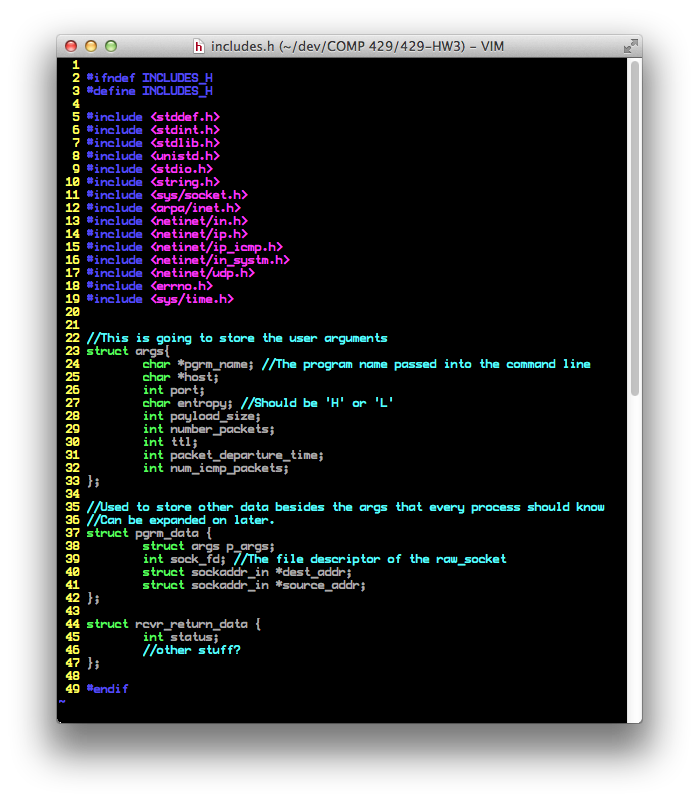
\includegraphics[scale=0.4]{images/includes-header.png}
\end{center}

\subsection{Sender}
\ \ \ \ We designated the Sender to stay on the main thread as this is the core of our project that requires the most attention from the operating system. The sender is broken up into two categories: send functions \textit{("sender.c")} and fill-out functions \textit{("network.c")}. The fill-out (or pack) functions simply take in a data structure (for example a \textit{struct ip} or \textit{struct udphdr}) and build it up. The send functions are responsible for taking the built-up structures and sending them.
\begin{center}
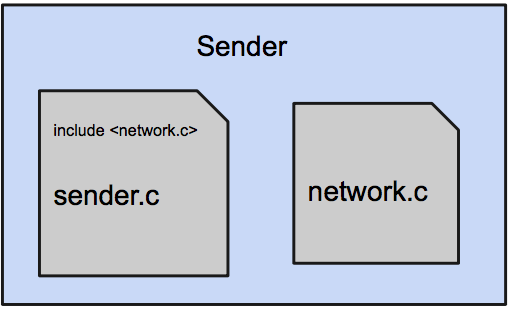
\includegraphics[scale=0.3]{images/sender-design.png}
\end{center}

\subsection{Receiver}
\ \ \ \ John-Luke Laue intended the Receiver to have the same design as the Sender, although he quickly realized that this was unnecessary as a result of unpacking not requiring a multitude of functions in order to work properly. Therefore, all Receiver functionality is in one file: \textit{("receiver.c")}. The main function,  \textit{receiver}, is the core of the Receiver which basically loops until it receives two icmp packets. There are only three small helper functions to help the receiver function (for example \textit{get\_icmp\_header} extracts the icmp packet from the ip datagram).
\begin{center}
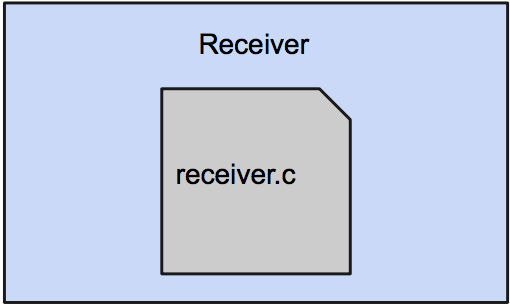
\includegraphics[scale=0.3]{images/receiver-design.png}
\end{center}

\section{Project Hindsight}
\ \ \ \ Splitting the sender, receiver, and network code made it easier to do parallel development, but it resulted in too many files. In addition, it was difficult to know what functions to make available to the sender and receiver threads. In the end, the Receiver didn't even use any functions outside of Receiver file. The interfaces for them ended up being a little clunky and did not do a good enough job of adding ease to creating messages, but it saved on lines of code.  Instead, we think that creating a function to simply take in the udp and icmp parameters and send the messages, rather than populating the message and returning it, would have been a better decision. This would have made the sender class easier to code, and further abstracted away from the networking. 
\ \ \ \ 

\section{Allocation of Work}
\ \ \ \ The collaborators of project collectively decided on how the work would be split up. The individuals of the team came up with different designs for the task, but we conjointly decided to capitalize on Jeffrey Limbacher's well-thought architecture. Upon general completion of the architecture design, we realized the significance of modularity in this project. Since there are two main hubs (the sender and the receiver) in this project, it made sense to assign at least one person per hub. John-Luke Laue was assigned the task of bringing together the receiver by himself, since this part was relatively straightforward. Varatep Buranintu and Jeffrey Limbacher modularly designed the sender hub and pooled resources together. Varatep Buranintu was responsible for the ICMP (head and tails) segment whilst Jeffrey Limbacher developed the UDP segment. Jeffrey Limbacher also built the raw socket and IP header as his tasks. Varatep Buranintu generated the project documentation and ensured the source code documentation (comments) is superlative so that another developer would be able to pick up where the project was left off.

\end{document}
